%!TEX root = ../larxxia.tex


\section{Laplace expansion theorem for determinants}
\label{sec:apd}
\secttoc


This section develops a so-called row\slash column algebraic expansion for determinants. 
This expansion is useful for many theoretical purposes.
But there are vastly more efficient ways of computing \idx{determinant}s than using a row\slash column expansion.  
In \script\ one may invoke \index{det()@\texttt{det()}}\verb|det(A)| to compute the determinant of a matrix.
You may find this function useful for checking the results of some examples and exercises.
However, just like computing an \idx{inverse}, computing the determinant is expensive and error prone.  
In medium to large scale problems avoid computing the determinant, something else is almost always better.

\begin{quoted}{\index{Moler, Cleve}Cleve Moler, MathWorks, 2006}
The most numerically reliable way to determine whether matrices are singular [not invertible] is to test their singular values. 
This is far better than trying to compute determinants, which have atrocious scaling properties.
\end{quoted}

Nonetheless, a row\slash column algebraic expansion for a determinant is useful for small matrix problems, as well as for its beautiful  theoretical uses.
We start with examples of row properties that underpin a row\slash column algebraic expansion.





\begin{example}[\autoref{thm:ppdet:i}] \label{eg:detzerorowii}
\autoref{eg:detzerorow} argued geometrically that the determinant is zero for the matrix
\begin{equation*}
A=\begin{bmatrix} 1&\frac12&0
\\0&\frac12&1 \\0&0&0 \end{bmatrix}.
\end{equation*}
Confirm this determinant algebraically.
\begin{solution} 
Using~\eqref{eq:dets23b}, \(\det A
=1\cdot\frac12\cdot0+\frac12\cdot1\cdot0+0\cdot0\cdot0
-0\cdot\frac12\cdot0-1\cdot1\cdot0-\frac12\cdot0\cdot0
=0\)\,.  
In every term there is a zero from the last row of the matrix.
\end{solution}
\end{example}


\begin{example}[\autoref{thm:ppdet:ii}] \label{eg:}
Consider the matrix with two identical rows,
\begin{equation*}
A=\begin{bmatrix} 1&\frac12&\frac15
\\1&\frac12&\frac15
\\0&\frac12&1 \end{bmatrix}.
\end{equation*}
Confirm algebraically that its determinant is zero.
Give a geometric reason for why its determinant has to be zero.

\begin{solution} 
Using~\eqref{eq:dets23b}, \(\det A =1\cdot\frac12\cdot1 +\frac12\cdot\frac15\cdot0 +\frac15\cdot1\cdot\frac12
-\frac15\cdot\frac12\cdot0 -1\cdot\frac15\cdot\frac12 -\frac12\cdot1\cdot1 =\frac12+\frac1{10}-\frac1{10}-\frac12=0\)\,.

%\Needspace{12ex}
%\begin{wrapfigure}{r}{0pt} % does not work in a list
%\ThreeD1{0.5}{0.2}1{0.5}{0.2}{0}{0.5}1
%\end{wrapfigure}
Geometrically, consider the image of the unit cube under multiplication by~\(A\) illustrated in stereo below. 
\begin{center}
\ThreeD1{0.5}{0.2}1{0.5}{0.2}{0}{0.5}1
\end{center}
Because the first two rows of~\(A\) are identical the first two components of~\(A\xv\) are always identical and hence all points are mapped onto the plane \(x_1=x_2\)\,.  
The image of the cube thus has zero thickness and hence zero volume.
By \autoref{def:detarea}, \(\det A=0\)\,.
\end{solution}
\end{example}




\begin{example}[\autoref{thm:ppdet:iii}] \label{eg:detswap}
Consider the two matrices with two rows swapped:
\begin{equation*}
A=\begin{bmatrix} 1&-1&0
\\0&1&1
\\\frac15&\frac12&1 \end{bmatrix},\qquad
B=\begin{bmatrix} 0&1&1
\\1&-1&0
\\\frac15&\frac12&1 \end{bmatrix}
\end{equation*}
Confirm algebraically that their determinants are the negative of each other.
Give a geometric reason why this should be so.
\begin{solution} 
Using~\eqref{eq:dets23b} twice: 
\begin{itemize}
\item \(\det A 
=1\cdot1\cdot1 +(-1)\cdot1\cdot\frac15 +0\cdot0\cdot\frac12
-0\cdot1\cdot\frac15 -1\cdot1\cdot\frac12 -(-1)\cdot0\cdot1 
=1-\frac15-\frac12=\frac3{10}\)\,;  
\item \(\det B =0\cdot(-1)\cdot1 
+1\cdot0\cdot\frac15 
+1\cdot1\cdot\frac12
-1\cdot(-1)\cdot\frac15 
-0\cdot0\cdot\frac12 
-1\cdot1\cdot1 
=\frac12+\frac15-1=-\frac3{10}=-\det A\)\,.
\end{itemize}
  

Geometrically, since the first two rows in~\(A\) and~\(B\) are swapped that means that multiplying by the matrix, as in \(A\xv\) and~\(B\xv\), has the first two components swapped.
Hence \(A\xv\) and~\(B\xv\) are always the reflection of each other in the plane \(x_1=x_2\).
%\marginpar{%
%\def\unithousesize{tiny}
%\def\unithouseviews{25,20}
%\ThreeD
%1{-1}{0}
%011
%{0.2}{0.5}1
%\\
%\ThreeD
%011
%1{-1}{0}
%{0.2}{0.5}1
%} %
Consequently, the images of the unit cubes under multiplication by~\(A\) and by~\(B\) are the reflection of each other in the plane \(x_1=x_2\)\,, as illustrated below,
and so the determinants must be the negative of each other.
\begin{center}
\def\unithouseviews{25,20}
\(A\)\quad\ThreeD
1{-1}{0}
011
{0.2}{0.5}1
\\
\(B\)\quad\ThreeD
011
1{-1}{0}
{0.2}{0.5}1
\end{center}
\end{solution}
\end{example}




\begin{example}[\autoref{thm:ppdet:iv}] \label{eg:}
Compute the determinant of the matrix
\begin{equation*}
B=\begin{bmatrix} 1&-1&0
\\0&1&1
\\2&5&10 \end{bmatrix}.
\end{equation*}
Compare~\(B\) with matrix~\(A\) given in \autoref{eg:detswap}, and compare their determinants.
\begin{solution} 
Using~\eqref{eq:dets23b}, \(\det B 
=1\cdot1\cdot10 +(-1)\cdot1\cdot2 +0\cdot0\cdot5
-0\cdot1\cdot2 -1\cdot1\cdot5 -(-1)\cdot0\cdot10 
=10-2-5=3\)\,.  
Matrix~\(B\) is the same as matrix~\(A\) except the third row is a factor of ten times bigger.
Correspondingly, \(\det B=3=10\times\frac3{10}=10\det A\)\,.
\end{solution}
\end{example}






The above four examples are specific cases of the four general properties established as the four parts of the following theorem. 


\begin{theorem}[row and column properties of determinants] \label{thm:ppdet} 
Let \(A\) be an \(n\times n\) matrix.
\begin{enumerate}
\item\label{thm:ppdet:i} 
If \(A\) has a \idx{zero row} or \index{zero column}column, then \(\det A=0\)\,.
\item\label{thm:ppdet:ii} 
If \(A\) has two \idx{identical rows} or \index{identical columns}columns, then  \(\det A=0\)\,.
\item\label{thm:ppdet:iii} 
Let \(B\) be obtained by \idx{interchanging two rows} or \index{interchanging two columns}columns of~\(A\), then \(\det B=-\det A\)\,.
\item\label{thm:ppdet:iv} 
Let \(B\) be obtained by multiplying any one row or column of~\(A\) by a scalar~\(k\), then \(\det B=k\det A\)\,.
\end{enumerate}
\end{theorem}

\begin{proof} 
We establish the  properties for matrix rows.  
Then the same property holds for the columns because \(\det(\tr A)=\det(A)\) (\autoref{thm:dettr}).
\begin{itemize}
\item[\ref{thm:ppdet:iv}]
Suppose row~\(i\) of matrix~\(A\) is multiplied by~\(k\) to give a new matrix~\(B\).
Let the diagonal matrix
\begin{equation*}
D:=\diag(1,\ldots,1,k,1,\ldots,1),
\end{equation*}
with the factor~\(k\) being in the \(i\)th~row and column.
Then \(\det D=1\times\cdots\times1\times k\times1\times\cdots\times1=k\)  by \autoref{thm:basicdet:i}.
Because multiplication by~\(D\) multiplies the \(i\)th~row by the factor~\(k\) and leaves everything else the same,  \(B=DA\)\,.
Equate determinants of both sides and use the product \autoref{thm:detprod}: \(\det B=\det(DA)=\det(D)\det(A)=k\det A\)\,.


\item[\ref{thm:ppdet:i}]
This arises from the case \(k=0\) of property~\ref{thm:ppdet:iv}.
Then \(A=DA\) because multiplying the \(i\)th~row of~\(A\) by \(k=0\) maintains that the row is zero.
Consequently, \(\det A=\det(DA)=\det(D)\det(A)=0\det(A)\) and hence \(\det A=0\)\,.

\item[\ref{thm:ppdet:iii}]
Suppose rows~\(i\) and~\(j\) of matrix~\(A\) are swapped to form matrix~\(B\).
Let the matrix~\(E\) be the identity except with rows~\(i\) and~\(j\) swapped:
\begin{equation*}
\begin{array}{rl}
E:=\begin{bmatrix} 
\ddots
\\&0&&1
\\&&\ddots
\\&1&&0
\\&&&&\ddots \end{bmatrix}&
\begin{matrix} \phantom{\vdots}
\\\text{row }i \\\phantom{\vdots}
\\\text{row }j \\\phantom{\vdots} \end{matrix}
\\
\begin{matrix}\phantom{\cdots}&i&\phantom{\cdots}&j&\phantom{\cdots}  \end{matrix}\quad&
\end{array}
\end{equation*}
where the diagonal dots~\(\ddots\) denote diagonals of ones, and all other entries of~\(E\) are zero.
Then \(B=EA\) as multiplication by~\(E\) copies row~\(i\) into row~\(j\) and vice versa.
Equate determinants of both sides and use \autoref{thm:detprod}: \(\det B=\det(EA)=\det(E)\det(A)\).

To find \(\det E\) observe that \(E\tr E=E^2=I_n\) so \(E\)~is orthogonal and hence \(\det E=\pm 1\) by \autoref{thm:basicdet:ii}.
Geometrically, multiplication by~\(E\) is a simple reflection in the $(n-1)$D-plane \(x_i=x_j\) hence its determinant must be negative, so \(\det E=-1\)\,.
Consequently, \(\det B=\det(E)\det(A)=-\det A\)\,.

\item[\ref{thm:ppdet:ii}]
Suppose rows~\(i\) and~\(j\) of matrix~\(A\) are identical.
Using the matrix~\(E\) to swap these two identical rows results in the same matrix: that is, \(A=EA\)\,.
Take determinants of both sides: \(\det A=\det(EA)=\det(E)\det(A)\).
Since \(\det E=-1\) it follows that \(\det A=-\det A\)\,.
Zero is the only number that equals its negative: thus \(\det A=0\)\,.
\end{itemize}
\end{proof}





\begin{example} \label{eg:}
You are given that \(\det A=-9\) for the matrix
\begin{equation*}
A=\begin{bmatrix}0&2&3&1&4
\\-2&2&-2&0&-3
\\4&-2&-4&1&0
\\2&-1&-4&2&2
\\5&4&3&-2&-5\end{bmatrix}.
\end{equation*}
Use \autoref{thm:ppdet} to find the determinant of the following matrices, giving reasons. 
\begin{parts}
\item \(\begin{bmatrix}0&2&3&0&4
\\-2&2&-2&0&-3
\\4&-2&-4&0&0
\\2&-1&-4&0&2
\\5&4&3&0&-5\end{bmatrix}\)
\begin{solution} 
\(\det=0\) as the fourth column is all zeros. 
\end{solution}

\item \(\begin{bmatrix}0&2&3&1&4
\\-2&2&-2&0&-3
\\2&-1&-4&2&2
\\4&-2&-4&1&0
\\5&4&3&-2&-5\end{bmatrix}\)
\begin{solution} 
\(\det=-\det A=+9\) as the 3rd and 4th rows are swapped. 
\end{solution}

\item \(\begin{bmatrix}0&2&3&1&4
\\-2&2&-2&0&-3
\\4&-2&-4&1&0
\\2&-1&-4&2&2
\\-2&2&-2&0&-3\end{bmatrix}\)
\begin{solution} 
\(\det=0\) as the 2nd and 5th rows are identical. 
\end{solution}

\item \(\begin{bmatrix}0&1&3&1&4
\\-2&1&-2&0&-3
\\4&-1&-4&1&0
\\2&-\frac12&-4&2&2
\\5&2&3&-2&-5\end{bmatrix}\)
\begin{solution} 
\(\det=\frac12\det A=-\frac92\) as the 2nd column is half that of~\(A\) 
\end{solution}

\item \(\begin{bmatrix}-2&2&-6&0&-3
\\4&-2&-12&1&0
\\2&-1&-12&2&2
\\0&2&9&1&4
\\5&4&9&-2&-5\end{bmatrix}\)
\begin{solution} 
\(\det=3(-\det A)=27\) as this matrix is~\(A\) with 1st and 4th rows swapped, and the 3rd column multiplied by~\(3\). 
\end{solution}

\item \(\begin{bmatrix}0&3&3&1&4
\\-2&0&-2&0&-5
\\5&-1&-4&1&0
\\2&-1&-4&2&2
\\5&4&6&-2&-5\end{bmatrix}\)
\begin{solution} 
Cannot answer as none of these row and column operations on~\(A\) appear to give this matrix.
\end{solution}

\end{parts}
% brute force search
%for i=1:99,a=round(randn(5)*3);if abs(det(a))<10, a=a,break,end,end
\end{example}




\begin{activity}
Now, \(\det\begin{bmatrix} 2&-3&1
\\2&-5&-3
\\-4&1&-3 \end{bmatrix}=-36\). 
\begin{itemize}
\item Which of the following matrices has determinant of~\(18\)?
\actposs{\(\begin{bmatrix} -1&-3&1
\\-1&-5&-3
\\2&1&-3 \end{bmatrix}\)}
{\(\begin{bmatrix} 2&-3&1
\\2&-5&-3
\\2&-5&-3 \end{bmatrix}\)}
{\(\begin{bmatrix} -4&6&-2
\\2&-5&-3
\\-4&1&-3 \end{bmatrix}\)}
{\(\begin{bmatrix} 2&-3&1/3
\\2&-5&-1
\\-4&1&-1 \end{bmatrix}\)}
%\begin{parts}
%\item \(\begin{bmatrix} -1&-3&1
%\\-1&-5&-3
%\\2&1&-3 \end{bmatrix}\)  \actans
%\item \(\begin{bmatrix} 2&-3&1
%\\2&-5&-3
%\\2&-5&-3 \end{bmatrix}\)
%\item \(\begin{bmatrix} -4&6&-2
%\\2&-5&-3
%\\-4&1&-3 \end{bmatrix}\)
%\item \(\begin{bmatrix} 2&-3&1/3
%\\2&-5&-1
%\\-4&1&-1 \end{bmatrix}\)
%\end{parts}
\item Further, which has determinant~\(-12\)? \(0\)? \(72\)?
\end{itemize}
\end{activity}



\begin{example} \label{eg:linedet}
Without evaluating the determinant, use \autoref{thm:ppdet} to establish that the determinant equation
\begin{equation}
\begin{vmatrix} 1&x&y\\1&2&3\\1&4&5 \end{vmatrix}=0
\label{eq:detline2}
\end{equation}
is the equation of the straight line in the \(xy\)-plane that passes through the two points~\((2,3)\) and~\((4,5)\).
\begin{solution} 
First, the determinant equation~\eqref{eq:detline2} is linear in variables \(x\) and~\(y\) as at most one of \(x\) and~\(y\) occur in each term of the determinant expansion:
\begin{center}\setlength{\unitlength}{1ex}
\begin{picture}(18,9)
%\put(0,0){\framebox(18,9){}}
{\color{red!50!white}\multiput(2.4,1)(3,0)3{\line(1,1)7}}
{\color{blue!50!white}\multiput(2.1,8)(3,0)3{\line(1,-1)7}}
\put(0,4){\(\begin{bmatrix} 1&x&y\\1&2&3\\1&4&5 \end{bmatrix}%
\begin{matrix} 1&x\\1&2\\1&4 \end{matrix}\)
}
%\thicklines
\end{picture}
\end{center}
Since the equation is linear in \(x\) and~\(y\), any solution set of~\eqref{eq:detline2} must be a straight line.
Second, equation~\eqref{eq:detline2} is satisfied when \((x,y)=(2,3)\) or when \((x,y)=(4,5)\) as then two rows in the determinant are identical, and so \autoref{thm:ppdet:ii} assures us the determinant is zero.
Thus the solution straight line passes through the two required points.

Let's evaluate the determinant to check:
equation~\eqref{eq:detline2} becomes
\(1\cdot2\cdot5 +x\cdot3\cdot1 +y\cdot1\cdot4 -y\cdot2\cdot1 -1\cdot3\cdot4 -x\cdot1\cdot5 =-2-2x+2y=0\)\,.  
That is, \(y=x+1\) which does indeed pass through \((2,3)\) and~\((4,5)\).
\end{solution}
\end{example}



\begin{example} \label{eg:planeq}
Without evaluating the determinant, use \autoref{thm:ppdet} to establish that the determinant equation
\begin{equation*}
\begin{vmatrix} x&y&z\\-1&-2&2\\3&5&2 \end{vmatrix}=0
\end{equation*}
is, in \(xyz\)-space, the equation of the plane that passes through the origin and the two points \((-1,-2,2)\) and~\((3,5,2)\).
\begin{solution} 
As in the previous example, the determinant is linear in~\(x\), \(y\) and~\(z\), so the solutions must be those of a single linear equation, namely a plane (\autoref{sec:nvep}).
\begin{itemize}
\item The solutions include the origin since when \(x=y=z=0\) the first row of the matrix is zero, hence the determinant is zero, and the equation satisfied.
\item The solutions include the  points \((-1,-2,2)\) and~\((3,5,2)\) since when \((x,y,z)\) is either of these points, then two rows in the determinant are identical, so the determinant is zero, and the equation satisfied.
\end{itemize}
Hence the solutions are the points in the plane passing through the origin and \((-1,-2,2)\) and~\((3,5,2)\).
\end{solution}
\end{example}






The next step in developing a general `formula' for a determinant is the special class of matrices for which one column or row is zero except for one element.


%\newcommand{\detpiciii}[9]{\setlength{\unitlength}{1ex}
%\begin{picture}(18,9)
%%\put(0,0){\framebox(18,9){}}
%\put(0,4){\ensuremath{\begin{bmatrix} 
%#1&#2&#3\\#4&#5&#6\\#7&#8&#9 \end{bmatrix}%
%\begin{matrix} #1&#2\\#4&#5\\#7&#8 \end{matrix}}
%}
%%\thicklines
%\color{red!50!white}\multiput(2,1)(3,0)3{\line(5,4)9}
%\color{blue!50!white}\multiput(2,8)(3,0)3{\line(5,-4)9}
%\end{picture}}

\begin{example} \label{eg:}
Find the determinant of 
\(A=\begin{bmatrix} -2&-1&-1\\1&-3&-2\\0&0&2 \end{bmatrix}\)
which has two zeros in its last row.
\begin{solution} Let's use two different arguments, both illustrating the next theorem and proof.
\begin{itemize}
\item Using~\eqref{eq:dets23b},
\begin{eqnarray*}
\det A&=& (-2)(-3)2+(-1)(-2)\cdot0+(-1)1\cdot0
\\&&{}
-(-1)(-3)0-(-2)(-2)0-(-1)1\cdot2
\\&=&2\big[(-2)(-3)-(-1)1\big]=2\cdot7=14\,.
\end{eqnarray*}
Observe \(\det A=2\times\det\begin{bmatrix} -2&-1\\1&-3 \end{bmatrix}\) which is the expression to be generalised.

\item Alternatively we use the product rule for determinants. Recognise that the matrix~\(A\) may be factored to \(A=FB\) where
\begin{equation*}
F=\begin{bmatrix} 1&0&-\frac12\\0&1&-1\\0&0&1 \end{bmatrix},
\quad B=\begin{bmatrix} -2&-1&0\\1&-3&0\\0&0&2 \end{bmatrix};
\end{equation*}
just multiply out and see that the last column of~\(F\) `fills in' the last column of~\(A\) from that of~\(B\).
Consider the geometry of the two transformations arising from multiplication by~\(F\) and by~\(B\).
\begin{itemize}
\item Multiplication by~\(F\) shears the unit cube as illustrated below.
\begin{center}
\ThreeD10{-0.5}01{-1}001
\end{center}
Thus the volume of the unit cube after multiplication by~\(F\) is the square base of area one, times the height of one, which is a volume of one.
Consequently \(\det F=1\) by \autoref{def:detarea}.

\item As illustrated  below, multiplication by~\(B\) has two components.
\begin{center}
\ThreeD{-2}{-1}01{-3}000{2}
\end{center}
Firstly,  the \(2\times2\) top-left sub-matrix, being bordered by zeros, maps the unit square in the \(x_1x_2\)-plane into the base parallelogram in the \(x_1x_2\)-plane.
The shape of the parallelogram is determined by the top-left sub-matrix \(\small\begin{bmatrix} -2&-1\\1&-3 \end{bmatrix}\) (to be called the \(A_{33}\)~minor) acting on the unit square.
Thus the area of the parallelogram is \(\det A_{33}=(-2)(-3)-(-1)1=7\)\,.
Secondly, the~\(2\) in the bottom corner of~\(B\) stretches objects vertically by a factor of~\(2\) to form a parallelepiped of height~\(2\).
Thus the volume of the parallelepiped is \(2\cdot\det A_{33}=2\cdot 7=14\)\,, which is \(\det B\) by \autoref{def:detarea}.

\end{itemize}
By the product \autoref{thm:detprod},
\(\det A=\det(FB)=\det(F)\det(B)=1\cdot14=14\)\,.

\end{itemize}
\end{solution}
\end{example}











\begin{theorem}[almost zero row/column] \label{thm:rpdet:vii} 
For every \(n\times n\) matrix~\(A\),
define the \((i,j)\)th~\bfidx{minor} \(A_{ij}\)~to be the \((n-1)\times(n-1)\) square matrix obtained from~\(A\) by omitting the \(i\)th~row and \(j\)th~column.  
If, except for the entry~\(a_{ij}\), the \(i\)th~row (or \(j\)th~column) of~\(A\) is all zero, then 
\begin{equation}
\det A=(-1)^{i+j}a_{ij}\det A_{ij}\,.
\label{eq:rpdet:vii}
\end{equation}
\end{theorem}
The pattern of signs in this formula,~\((-1)^{i+j}\), is 
\begin{equation*}
\begin{matrix} +&-&+&-&+&\cdots
\\-&+&-&+&-&\cdots
\\+&-&+&-&+&\cdots
\\-&+&-&+&-&\cdots
\\+&-&+&-&+&\cdots
\\\vdots&\vdots&\vdots&\vdots&\vdots&\ddots \end{matrix}
\end{equation*}

\begin{proof} 
We establish the determinant formula~\eqref{eq:rpdet:vii} for matrix rows,  then the same result holds for the columns because \(\det(\tr A)=\det(A)\) (\autoref{thm:dettr}).
First, if the entry~\(a_{ij}=0\)\,, then the whole \(i\)th~row (or \(j\)th~column) is zero and so \(\det A=0\) by \autoref{thm:ppdet:i}.  
Also, the expression \((-1)^{i+j}a_{ij}\det A_{ij}=0\) as \(a_{ij}=0\)\,.  
Consequently, the identity \(\det A=(-1)^{i+j}a_{ij}\det A_{ij}\) holds.
The rest of this proof addresses the case \(a_{ij}\neq 0\)\,.

Second, consider the special case when the last row \emph{and} last column of matrix~\(A\) is all zero except for~\(a_{nn}\neq0\); that is, 
\begin{equation*}
A=\begin{bmatrix} A_{nn}&\ov\\\tr\ov&a_{nn} \end{bmatrix}
\end{equation*}
for the minor~\(A_{nn}\) and \(\ov\in\RR^{n-1}\).
\marginpar{%
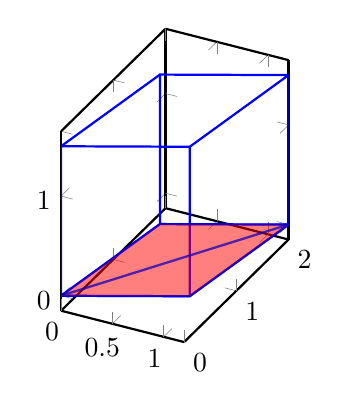
\begin{tikzpicture}
\def\a{1} \def\b{0.2} \def\c{0}
\def\d{0.5} \def\e{1.5} \def\f{0}
\def\g{0} \def\h{0} \def\i{1.5}
\begin{axis}[ view={27}{30}
%  ,\footnotesize % this size seems to break it for some reason
%  ,xlabel={$x_1$}, ylabel={$x_2$}, zlabel={$x_3$}
  ,thick,axis equal image ,no marks %,grid
  ] 
\addplot3[blue] coordinates {(0,0,0) (\a,\d,\g)
%  (\a+0.4*\b,\d+0.4*\e,\g+0.4*\h)
%  (\a+0.4*\b+0.6*\c,\d+0.4*\e+0.6*\f,\g+0.4*\h+0.6*\i)
%  (\a+0.7*\b+0.6*\c,\d+0.7*\e+0.6*\f,\g+0.7*\h+0.6*\i)
%  (\a+0.7*\b,\d+0.7*\e,\g+0.7*\h)% doorway
  (\a+\b,\d+\e,\g+\h)
  (\b,\e,\h) (0,0,0) (\c,\f,\i) (\a+\c,\d+\f,\g+\i)
%  (0.5*\a+0.5*\b+1.2*\c,0.5*\d+0.5*\e+1.2*\f,0.5*\g+0.5*\h+1.2*\i)
  (\c,\f,\i)  (\b+\c,\e+\f,\h+\i) 
%  (0.5*\a+0.5*\b+1.2*\c,0.5*\d+0.5*\e+1.2*\f,0.5*\g+0.5*\h+1.2*\i)
  (\a+\b+\c,\d+\e+\f,\g+\h+\i) (\b+\c,\e+\f,\h+\i)
  (\b,\e,\h) (\a+\b,\d+\e,\g+\h) (\a+\b+\c,\d+\e+\f,\g+\h+\i)
  (\a+\c,\d+\f,\g+\i) (\a,\d,\g)
  }; 
\addplot3[patch,red,opacity=0.5] coordinates {
  (0,0,0) (\a,\d,\g) (\a+\b,\d+\e,\g+\h) 
  (\a+\b,\d+\e,\g+\h) (\b,\e,\h) (0,0,0)};
\end{axis}
\end{tikzpicture}}
Recall \autoref{def:detarea}: the image of the \(n\)D-cube under multiplication by the matrix~\(A\) is the image of the \((n-1)\)D-cube under multiplication by~\(A_{nn}\) extended orthogonally a length~\(a_{nn}\) in the orthogonal direction~\(\ev_n\) (as illustrated in the margin in 3D).
The volume of the \(n\)D-image is thus \(a_{nn}\times{}\)(volume of the \((n-1)\)D-image).
Consequently, \(\det A=a_{nn}\det A_{nn}\)\,.
\begin{comment}
The above glosses over details for when \(a_{nn}<0\).
\end{comment}

Third, consider the special case when the last row of matrix~\(A\) is all zero except for~\(a_{nn}\neq0\); that is, 
\begin{equation*}
A=\begin{bmatrix} A_{nn}&\av_n'\\\tr\ov&a_{nn} \end{bmatrix}
\end{equation*}
for the minor~\(A_{nn}\), and where \(\av'_n=(a_{1n},a_{2n},\ldots,a_{n-1,n})\).
Define the two \(n\times n\)~matrices
\begin{equation*}
F:=\begin{bmatrix} I_{n-1}&\av'_n/a_{nn}\\\tr\ov& 1 \end{bmatrix}
\quad\text{and }
B:=\begin{bmatrix} A_{nn}&\ov\\\tr\ov&a_{nn} \end{bmatrix}.
\end{equation*}
Then \(A=FB\) since
\begin{eqnarray*}
FB&=&\begin{bmatrix} I_{n-1}&\av'_n/a_{nn}\\\tr\ov& 1 \end{bmatrix}
\begin{bmatrix} A_{nn}&\ov\\\tr\ov&a_{nn} \end{bmatrix}
\\&=&\begin{bmatrix} I_{n-1}A_{nn}+\av'_n/a_{nn}\tr\ov &
I_{n-1}\ov+\av'_n/a_{nn}\cdot a_{nn}\\
\tr\ov A_{nn}+1\cdot\tr\ov &
\tr\ov\ov+1\cdot a_{nn}  \end{bmatrix}
\\&=&\begin{bmatrix} A_{nn} &
\av'_n\\
\tr\ov  &
a_{nn}  \end{bmatrix} =A\,.
\end{eqnarray*}
By \autoref{thm:detprod}, \(\det A=\det(FB)=\det(F)\det(B)\)\,.
From the previous part \(\det B=a_{nn}\det A_{nn}\)\,, so we just need to determine~\(\det F\)\,.
\marginpar{\def\unithouseviews{30}\ThreeD10{0.5}01{0.4}001}
As illustrated for 3D in the margin, the action of matrix~\(F\) on the unit \(n\)D-cube is that of a simple shear keeping the \((n-1)\)D-cube base unchanged (due to the identity~\(I_{n-1}\) in~\(F\)).
Since the height orthogonal to the \((n-1)\)D-cube base is unchanged (due to the one in the bottom-right corner of~\(F\)), the action of multiplying by~\(F\) leaves the volume of the unit \(n\)D-cube unchanged at one.
Hence \(\det F=1\)\,.
Thus \(\det A=1\det(B)=a_{nn}\det A_{nn}\) as required.

Fourth, suppose row~\(i\) of matrix~\(A\) is all zero except for entry~\(a_{ij}\).
Swap rows~\(i\) and~\(i+1\), then swap rows~\(i+1\) and~\(i+2\), and so on until the original row~\(i\) is in the last row, and the order of all other rows are unchanged: this takes \((n-i)\)~row swaps which changes the sign of the determinant \((n-i)\)~times (\autoref{thm:ppdet:iii}), that is, multiplies it by~\((-1)^{n-i}\).
Then swap columns~\(j\) and~\(j+1\), then swap columns~\(j+1\) and~\(j+2\), and so on until the original column~\(j\) is in the last column: this takes \((n-j)\)~column swaps which change the determinant by a factor~\((-1)^{n-j}\) (\autoref{thm:ppdet:iii}).
The resulting matrix, say~\(C\), has the form
\begin{equation*}
C=\begin{bmatrix} A_{ij}&\av'_j\\\tr\ov&a_{ij} \end{bmatrix}
\end{equation*}
for \(\av'_j\) denoting the \(j\)th~column of~\(A\) with the \(i\)th~entry omitted.
Since matrix~\(C\) has the form addressed in the first part, we know \(\det C=a_{ij}\det A_{ij}\)\,.
From the row and column swapping, \(\det A=(-1)^{n-i}(-1)^{n-j}\det C =(-1)^{2n-i-j}\det C =(-1)^{-(i+j)}\det C =(-1)^{i+j}\det C =(-1)^{i+j}a_{ij}\det A_{ij}\)\,.
\end{proof}




\begin{example} \label{eg:rpdet}
Use \autoref{thm:rpdet:vii} to evaluate the determinant of the following matrices.  
\begin{parts}
\item \(\begin{bmatrix} -3&-3&-1\\-3&2&0\\0&0&2 \end{bmatrix}\)
\begin{solution} 
There are two zeros in the bottom row so the determinant is \((-1)^62\det\begin{bmatrix} -3&-3\\-3&2 \end{bmatrix}=2(-6-9)=-30\)\,. 
\end{solution}

\item \(\begin{bmatrix} 2&-1&7\\0&3&0\\2&2&5 \end{bmatrix}\)
\begin{solution} 
There are two zeros in the middle row so the determinant is \((-1)^43\det\begin{bmatrix} 2&7\\2&5 \end{bmatrix}=3(10-14)=-12\)\,. 
\end{solution}

\item \(\begin{bmatrix} 2&4&3\\8&0&-1\\-5&0&-2 \end{bmatrix}\)
\begin{solution} 
There are two zeros in the middle column so the determinant is \((-1)^34\det\begin{bmatrix} 8&-1\\-5&-2 \end{bmatrix}=-4(-16-5)=84\)\,. 
\end{solution}

\item \(\begin{bmatrix} 2&1&3\\0&-2&-3\\0&2&4 \end{bmatrix}\)
\begin{solution} 
There are two zeros in the first column so the determinant is \((-1)^22\det\begin{bmatrix} -2&-3\\2&4 \end{bmatrix}=2(-8+6)=-4\)\,. 
\end{solution}

\end{parts}
%\begin{comment}
%\begin{verbatim}
%a=round(randn(3)*3);i=ceil(3*rand(1,2));a((1:3)~=i(2),i(1))=0,det(a)
%\end{verbatim}
%\end{comment}
\end{example}




\begin{activity}
Using one of the determinants in the above \autoref{eg:rpdet}, what is the determinant of the matrix
\begin{equation*}
\begin{bmatrix} 2&1&0&3
\\5&-2&15&2
\\0&-2&0&-3
\\0&2&0&4 \end{bmatrix} ?
\end{equation*}
\actposs[4]{\(60\)}{\(-120\)}{\(-60\)}{\(120\)}
%\partswidth=5em
%\begin{parts}
%\item \(-120\)
%\item \(-60\)
%\item \(60\)\actans
%\item \(120\)
%\end{parts}
\end{activity}






\begin{example} \label{eg:dettrii}
Use \autoref{thm:rpdet:vii} to evaluate the determinant of the  so-called \idx{triangular matrix}  
%a=triu(round(randn(5)*3))
\begin{equation*}
A=\begin{bmatrix}2&-2&3&1&0
\\0&2&-1&-1&-7
\\0&0&5&-2&-9
\\0&0&0&1&1
\\0&0&0&0&3 \end{bmatrix}
\end{equation*}
\begin{solution} 
The last row is all zero except for the last element of~\(3\), so
\begin{eqnarray*}
\det A&=&(-1)^{10}3\det\begin{bmatrix}2&-2&3&1
\\0&2&-1&-1
\\0&0&5&-2
\\0&0&0&1\end{bmatrix}
\\&&(\text{then as the last row is zero except the~\(1\)})
\\&=&3\cdot (-1)^81\det\begin{bmatrix}2&-2&3
\\0&2&-1
\\0&0&5\end{bmatrix}
\\&&(\text{then as the last row is zero except the~\(5\)})
\\&=&3\cdot1\cdot(-1)^65\det\begin{bmatrix}2&-2
\\0&2\end{bmatrix}
\\&&(\text{then as the last row is zero except the~\(2\)})
\\&=&3\cdot1\cdot5(-1)^42\det\begin{bmatrix}2\end{bmatrix}
\\&=&3\cdot1\cdot5\cdot2\cdot2=60\,.
\end{eqnarray*}
\end{solution}
\end{example}


The relative simplicity of finding the determinant in \autoref{eg:dettrii} indicates that there is something special and memorable about matrices with zeros in the entire lower-left `triangle'.
There is, as expressed by the following definition and theorem.






\begin{definition} \label{def:trim}
A \bfidx{triangular matrix} is a \idx{square matrix} where all entries are zero either to the lower-left of the diagonal or to the upper-right:
\footnote{From time-to-time, some people call an upper triangular matrix either a \idx{right triangular} or an \idx{upper-right triangular} matrix.  
Correspondingly, from time-to-time, some people  call a lower triangular matrix either a \idx{left triangular} or a \idx{lower-left triangular} matrix.}
\begin{itemize}
\item an \idx{upper triangular} matrix has the form (although any of the~\(a_{ij}\) may also be zero)
\begin{equation*}
\begin{bmatrix} a_{11}&a_{12}&\cdots&a_{1\,n-1}&a_{1n}
\\0&a_{22}&\cdots&a_{2\,n-1} &a_{2n}
\\\vdots&0&\ddots&\vdots&\vdots
\\0&\vdots&\ddots&a_{n-1\,n-1}&a_{n-1\,n} 
\\0&0&\cdots&0&a_{nn} \end{bmatrix};
\end{equation*}

\item a \idx{lower triangular} matrix has the form (although any of the~\(a_{ij}\) may also be zero)
\begin{equation*}
\begin{bmatrix} a_{11}&0&\cdots&0&0
\\a_{21}&a_{22}&0&\cdots &0
\\\vdots&\vdots&\ddots&\ddots&\vdots
\\a_{n-1\,1}&a_{n-1\,2}&\cdots&a_{n-1\,n-1}&0 
\\a_{n\,1}&a_{n\,2}&\cdots&a_{n\,n-1}&a_{n\,n} \end{bmatrix}.
\end{equation*}
\end{itemize}
\end{definition}


Any square \idx{diagonal matrix} is also an upper triangular matrix, and also a lower triangular matrix.
Thus the following theorem encompasses square diagonal matrices and so generalises \autoref{thm:basicdet:i}.



\begin{theorem}[triangular matrix]\label{thm:rpdet:vi} 
For every \(n\times n\) \idx{triangular matrix}~\(A\),
the \idx{determinant} of~\(A\) is the product of the diagonal entries, \(\det A=a_{11}a_{22}\cdots a_{nn}\).
\end{theorem}
\begin{proof} 
A little induction proves the determinant of a triangular matrix is the product of its diagonal entries: only consider upper triangular matrices as transposing the matrix caters for lower triangular matrices.

First, for \(1\times 1\) matrices the result is trivial.
The results is also straightforward for \(2\times 2\) matrices since the determinant
\begin{equation*}
\begin{vmatrix} a_{11}&a_{12}\\0&a_{22} \end{vmatrix}
=a_{11}a_{22}-0a_{12}=a_{11}a_{22}
\end{equation*}
which is the product of the diagonal entries as required.

Second, assume the property for \((n-1)\times(n-1)\) matrices.
Now, every upper triangular \(n\times n\) matrix~\(A\) has the form
\begin{equation*}
A=\begin{bmatrix} A_{nn}&\av_n'\\\tr\ov&a_{nn} \end{bmatrix}.
\end{equation*}
for \((n-1)\times(n-1)\) minor~\(A_{nn}\).
\autoref{thm:rpdet:vii} establishes \(\det A=a_{nn}\det A_{nn}\)\,.  
Since the  minor~\(A_{nn}\) is upper triangular and \((n-1)\times(n-1)\), by assumption \(\det A_{nn}=a_{11}a_{22}\cdots a_{n-1,n-1}\)\,.
Consequently, \(\det A=a_{nn}\det A_{nn}=a_{nn}a_{11}a_{22}\cdots a_{n-1,n-1}\)\,, as required.
Induction then establishes the theorem for all~\(n\).
\end{proof}




\begin{activity}
Which of the following matrices is \emph{not} a triangular matrix?
\actposs{\(\begin{bmatrix} 0&0&0&-2
\\0&0&-1&-1
\\0&1&1&4
\\-1&-1&0&3 \end{bmatrix}\)}
{\(\begin{bmatrix} -1&-1&1&0
\\0&-5&4&2
\\0&0&1&-2
\\0&0&0&1 \end{bmatrix}\)}
{\(\begin{bmatrix} 0&0&0&0
\\3&4&0&0
\\4&-2&-1&0
\\-1&-2&2&-3 \end{bmatrix}\)}
{\(\begin{bmatrix} -2&0&0&0
\\0&-1&0&0
\\0&0&2&0
\\0&0&0&3 \end{bmatrix}\)}
%\begin{parts}
%\item \(\begin{bmatrix} -1&-1&1&0
%\\0&-5&4&2
%\\0&0&1&-2
%\\0&0&0&1 \end{bmatrix}\)
%\item \(\begin{bmatrix} 0&0&0&0
%\\3&4&0&0
%\\4&-2&-1&0
%\\-1&-2&2&-3 \end{bmatrix}\)
%\item \(\begin{bmatrix} 0&0&0&-2
%\\0&0&-1&-1
%\\0&1&1&4
%\\-1&-1&0&3 \end{bmatrix}\)
%\item \(\begin{bmatrix} -2&0&0&0
%\\0&-1&0&0
%\\0&0&2&0
%\\0&0&0&3 \end{bmatrix}\)
%\end{parts}
\end{activity}




\begin{example} \label{eg:}
Find the determinant of those of the following matrices which are triangular.
%a=triu(round(randn(5)*3))
\begin{enumerate}
\item \(\begin{bmatrix}-1&-1&-1&-5
\\0&-4&1&4
\\0&0&7&0
\\0&0&0&-3 \end{bmatrix}\)
\begin{solution} 
This is upper triangular, and its determinant is \((-1)\cdot(-4)\cdot7\cdot(-3)=-84\). 
\end{solution}

\item \(\begin{bmatrix}-3&0&0&0
\\-4&2&0&0
\\-1&1&1&0
\\-2&-3&7&-1\end{bmatrix}\)
\begin{solution} 
This is lower triangular, and its determinant is \((-3)\cdot2\cdot1\cdot)-1)=6\). 
\end{solution}

\item \(\begin{bmatrix}-4&0&0&0
\\2&-2&0&0
\\-5&-3&-2&0
\\-2&5&-2&0\end{bmatrix}\)
\begin{solution} 
This is lower triangular, and its determinant is zero as it has a column of zeros. 
\end{solution}

\item \(\begin{bmatrix}0.2&0&0&0
\\0&1.1&0&0
\\0&0&-0.5&0
\\0&0&0&0.9\end{bmatrix}\)
\begin{solution} 
This diagonal matrix is both upper and lower triangular, and its determinant is \(0.2\cdot1.1\cdot(-0.5)\cdot0.9=-0.099\). 
\end{solution}

%a=triu(round(randn(4)*3)),a=a(randperm(4),:)
\item \(\begin{bmatrix}1&-1&1&-3
\\0&0&0&-5
\\0&0&-3&-4
\\0&-2&1&-2\end{bmatrix}\)
\begin{solution} 
This is not triangular, so we do not have to compute its determinant. 
Nonetheless, if we swap the 2nd and 4th~rows, then the result is the upper triangular \(\footnotesize\begin{bmatrix}1&-1&1&-3
\\0&-2&1&-2
\\0&0&-3&-4
\\0&0&0&-5\end{bmatrix}\) and its determinant is \(1\cdot(-2)\cdot(-3)\cdot(-5)=-30\). 
But the row swap changes the sign so the determinant of the original matrix is~\(-(-30)=30\).
\end{solution}

\item \(\begin{bmatrix}0&0&0&-3
\\0&0&2&-4
\\0&-1&4&-1
\\-6&1&5&1\end{bmatrix}\)
\begin{solution} 
This is \emph{not} triangular, so we do not have to compute its determinant. 
Nonetheless, if we swap the 1st and 4th~rows, and the 2nd and 3rd~rows, then the result is the lower triangular \(\footnotesize\begin{bmatrix}-3&0&0&0
\\-4&2&0&0
\\-1&4&-1&0
\\1&5&1&-6\end{bmatrix}\) and its determinant is \((-3)\cdot2\cdot(-1)\cdot(-6)=-36\). 
But each row swap changes the sign so the determinant of the original matrix is~\((-1)^2(-36)=-36\). 
\end{solution}

\item \(\begin{bmatrix}-1&0&0&1
\\-2&0&0&0
\\2&-2&-1&-2
\\-1&0&4&2\end{bmatrix}\)
\begin{solution} 
This is not triangular, so we do not have to compute its determinant. 
Nonetheless, if we magically know to swap the 2nd and 4th~columns, the 1st and 2nd~rows, and the 3rd and 4th~rows, then the result is the lower triangular \(\footnotesize\begin{bmatrix}-2&0&0&0
\\-1&1&0&0
\\-1&2&4&0
\\2&-2&-1&-2\end{bmatrix}\) and its determinant is \((-2)\cdot1\cdot4\cdot(-2)=16\). 
But each row and column swap changes the sign so the determinant of the original matrix is~\((-1)^316=-16\). 
\end{solution}
\end{enumerate}
\end{example}



The above case of triangular matrices is a short detour from the main development of this section which is to derive a formula for determinants in general.
The following two examples introduce the next property we need before establishing a general formula for determinants.


\begin{example} \label{eg:}
Let's rewrite the explicit formulas~\eqref{eq:dets23b} for \(2\times2\) and \(3\times3\) determinants explicitly as the sum of simpler determinants.
\begin{itemize}
\item Recall that the \(2\times2\) determinant
\begin{eqnarray*}
\begin{vmatrix} a&b\\c&d \end{vmatrix}
&=&ad-bc
\\&=&(ad-0c)+(0d-bc)
\\&=&\begin{vmatrix} a&0\\c&d \end{vmatrix}
+\begin{vmatrix} 0&b\\c&d \end{vmatrix}.
\end{eqnarray*}
That is, the original determinant is the same as the sum of two determinants, each with a zero in the first row and the other row unchanged.
This identity decomposes the first row as \(\begin{bmatrix} a&b \end{bmatrix}=\begin{bmatrix} a&0 \end{bmatrix}+\begin{bmatrix} 0&b \end{bmatrix}\), while the other row is unchanged.

\item Recall from~\eqref{eq:dets23b} that the \(3\times3\) determinant
\begin{eqnarray*}
\begin{vmatrix} a&b&c\\d&e&f\\g&h&i \end{vmatrix}
&=&\phantom{{}+}aei+bfg+cdh-ceg-afh-bdi
\\&=&{}+aei+0fg+0dh-0eg-afh-0di
\\&&{}+0ei+bfg+0dh-0eg-0fh-bdi
\\&&{}+0ei+0fg+cdh-ceg-0fh-0di
\\&=&\begin{vmatrix} a&0&0\\d&e&f\\g&h&i \end{vmatrix}
+\begin{vmatrix} 0&b&0\\d&e&f\\g&h&i \end{vmatrix}
+\begin{vmatrix} 0&0&c\\d&e&f\\g&h&i \end{vmatrix}.
\end{eqnarray*}
That is, the original determinant is the same as the sum of three determinants, each with two zeros in the first row and the other rows unchanged.
This identity decomposes the first row as \(\begin{bmatrix} a&b&c \end{bmatrix}=\begin{bmatrix} a&0&0 \end{bmatrix}+\begin{bmatrix} 0&b&0 \end{bmatrix}+\begin{bmatrix} 0&0&c \end{bmatrix}\), while the other rows are unchanged.
\end{itemize}
This sort of rearrangement of a determinant makes progress because then \autoref{thm:rpdet:vii} helps by finding the determinant of the resultant matrices that have an almost all zero row.
\end{example}

\begin{example} \label{eg:cpdet2}
A \(2\times2\) example of a more general summation property is furnished by the determinant of matrix \(A=\begin{bmatrix} a_{11}&b_1+c_1\\a_{21}&b_2+c_2 \end{bmatrix}\).
\begin{eqnarray*}
\det A&=&a_{11}(b_2+c_2)-a_{21}(b_1+c_1)
\\&=&a_{11}b_2+a_{11}c_2-a_{21}b_1-a_{21}c_1
\\&=&(a_{11}b_2-a_{21}b_1)+(a_{11}c_2-a_{21}c_1)
\\&=&\det\begin{bmatrix} a_{11}&b_1\\a_{21}&b_2 \end{bmatrix}
+\det\begin{bmatrix} a_{11}&c_1\\a_{21}&c_2 \end{bmatrix}
\\&=&\det B+\det C\,,
\end{eqnarray*}
where matrices~\(B\) and~\(C\) have the same first column as~\(A\), and their second columns add up to the second column of~\(A\).
\end{example}





\begin{theorem}[sum formula] \label{thm:rpdet:v} 
Let \(A\), \(B\) and~\(C\) be \(n\times n\) matrices.
If matrices~\(A\), \(B\) and~\(C\) are identical except for their \(i\)th~column, and that the \(i\)th~column of~\(A\) is the sum of the \(i\)th~columns of \(B\) and~\(C\), then \(\det A=\det B+\det C\)\,.
Further, the same sum property holds when ``column'' is replaced by ``row'' throughout.
\end{theorem}


\begin{proof} 
We establish the theorem for matrix columns.
Then the same results holds for the rows because \(\det(\tr A)=\det(A)\) (\autoref{thm:dettr}).
As a prelude to the general geometric proof, consider the \(2\times 2\) case and the second column (as also established algebraically by \autoref{eg:cpdet2}).  
Write the matrices in terms of their column vectors, and draw the determinant parallelogram areas as shown  below: let
\def\a{2.5} \def\b{0.5} \def\ab{3}
\def\c{0.5} \def\d{1.7} \def\cd{2.2}
\def\bi{1} \def\abi{3.5}
\def\di{1} \def\cdi{1.5}
\def\bj{-0.5} \def\abj{2}
\def\dj{0.7}  \def\cdj{1.2}
\begin{eqnarray*}
A=\begin{bmatrix} \av_1&\av_2 \end{bmatrix},
&&
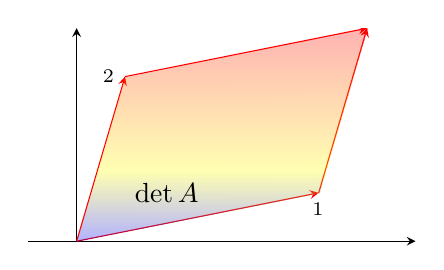
\begin{tikzpicture} 
\begin{axis}[small,axis equal image
    , axis lines=middle
    ,xtick={0},xticklabels={$0$}
    ,ytick={0},yticklabels={$0$}
    ,xmin=-0.5,xmax=3.5,ymax=2.2
    ]
    \addplot[quiver={u=\a,v=\c},red,-stealth] coordinates {(0,0)(\b,\d)};
    \node[below] at (axis cs:\a,\c) {$\av_1$};
    \addplot[quiver={u=\b,v=\d},red,-stealth] coordinates {(0,0)(\a,\c)};
    \node[left] at (axis cs:\b,\d) {$\av_2$};
\addplot[patch,opacity=0.3,shader=interp] coordinates {
(0,0) (\a,\c) (\b,\d)
(\ab,\cd) (\b,\d)  (\a,\c)
};
    \node[right] at (axis cs:\b,\c) {$\det A$};
\end{axis}
\end{tikzpicture}
\\
B=\begin{bmatrix} \av_1&\bv \end{bmatrix},
&&
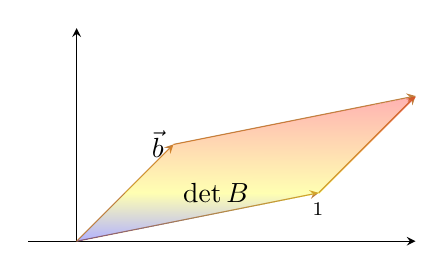
\begin{tikzpicture} 
\begin{axis}[small,axis equal image
    , axis lines=middle
    ,xtick={0},xticklabels={$0$}
    ,ytick={0},yticklabels={$0$}
    ,xmin=-0.5,xmax=3.5,ymax=2.2
    ]
    \addplot[quiver={u=\a,v=\c},brown,-stealth] coordinates {(0,0)(\bi,\di)};
    \node[below] at (axis cs:\a,\c) {$\av_1$};
    \addplot[quiver={u=\bi,v=\di},brown,-stealth] coordinates {(0,0)(\a,\c)};
    \node[left] at (axis cs:\bi,\di) {$\vec b$};
\addplot[patch,opacity=0.3,shader=interp] coordinates {
(0,0) (\a,\c) (\bi,\di)
(\abi,\cdi) (\bi,\di)  (\a,\c)
};
    \node[right] at (axis cs:\bi,\c) {$\det B$};
\end{axis}
\end{tikzpicture}
\\
C=\begin{bmatrix} \av_1&\cv \end{bmatrix},
&&
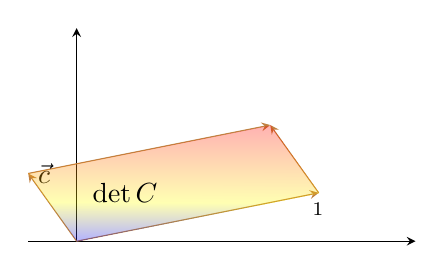
\begin{tikzpicture} 
\begin{axis}[small,axis equal image
    , axis lines=middle
    ,xtick={0},xticklabels={$0$}
    ,ytick={0},yticklabels={$0$}
    ,xmin=-0.5,xmax=3.5,ymax=2.2
    ]
    \addplot[quiver={u=\a,v=\c},brown,-stealth] coordinates {(0,0)(\bj,\dj)};
    \node[below] at (axis cs:\a,\c) {$\av_1$};
    \addplot[quiver={u=\bj,v=\dj},brown,-stealth] coordinates {(0,0)(\a,\c)};
    \node[right] at (axis cs:\bj,\dj) {$\vec c$};
\addplot[patch,opacity=0.3,shader=interp] coordinates {
(0,0) (\a,\c) (\bj,\dj)
(\abj,\cdj) (\bj,\dj)  (\a,\c)
};
    \node at (axis cs:0.5,\c) {$\det C$};
\end{axis}
\end{tikzpicture}
\end{eqnarray*}
The matrices \(A\), \(B\) and~\(C\) all have the same first column~\(\av_1\), whereas the second columns satisfy \(\av_2=\bv+\cv\) by the condition of the theorem. 
Because these parallelograms have common side~\(\av_1\) we can stack the area for \(\det C\) on top of that for~\(\det B\), and because \(\av_2=\bv+\cv\) the top edge of the stack matches that for the area~\(\det A\), as shown below
\begin{center}
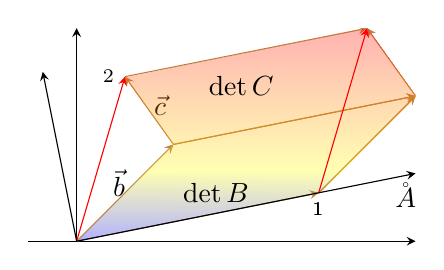
\begin{tikzpicture} 
\begin{axis}[small,axis equal image
    , axis lines=middle
    ,xtick={0},xticklabels={$0$}
    ,ytick={0},yticklabels={$0$}
    ,xmin=-0.5,xmax=3.5,ymax=2.2
    ]
    \addplot[quiver={u=\a,v=\c},brown,-stealth] coordinates {(0,0)(\bi,\di)};
    \node[below] at (axis cs:\a,\c) {$\av_1$};
    \addplot[quiver={u=\bi,v=\di},brown,-stealth] coordinates {(0,0)(\a,\c)};
    \node[left] at (axis cs:0.6,0.6) {$\vec b$};
    \addplot[quiver={u=\a,v=\c},brown,-stealth] 
    coordinates {(\bi,\di)(\bi+\bj,\di+\dj)};
    \node[below] at (axis cs:\a,\c) {$\av_1$};
    \addplot[quiver={u=\bj,v=\dj},brown,-stealth] 
    coordinates {(\bi,\di)(\bi+\a,\di+\c)};
    \node[right] at (axis cs:0.7,1.4) {$\vec c$};
\addplot[patch,opacity=0.3,shader=interp] coordinates {
(0,0) (\a,\c) (\bi,\di)
(\abi,\cdi) (\bi,\di)  (\a,\c)
(\bi,\di) (\bi+\a,\di+\c) (\bi+\bj,\di+\dj)
(\bi+\abj,\di+\cdj) (\bi+\bj,\di+\dj)  (\bi+\a,\di+\c)
};
    \node[right] at (axis cs:\bi,\c) {$\det B$};
    \node at (axis cs:1.7,1.6) {$\det C$};
    \addplot[quiver={u=\b,v=\d},red,-stealth] coordinates {(0,0) (\a,\c)};
    \node[left] at (axis cs:\b,\d) {$\av_2$};
% orthog axes
\addplot[quiver={u=\a*1.4,v=\c*1.4},black,-stealth] coordinates {(0,0)};
\addplot[quiver={u=-\c*0.7,v=\a*0.7},black,-stealth] coordinates {(0,0)};
\node[below] at (axis cs:3.4,0.7) {$\AA$};
\node[left] at (axis cs:-0.2,1) {$\nv$};
\end{axis}
\end{tikzpicture}
\end{center}
The base of the stacked shape lies on the line~\AA, and let vector~\nv\ denote the orthogonal\slash normal direction (as shown).
Because the shape has the same cross-section in lines parallel to~\AA, its area is the area of the base times the height of the stacked shape in the direction~\nv.
But this is precisely the same height and base as the area for~\(\det A\), hence \(\det A=\det B+\det C\)\,.

A general proof for the last column uses the same diagrams, albeit schematically. 
Let matrices
\begin{equation*}
A=\begin{bmatrix} A'& \av_n \end{bmatrix},\quad
B=\begin{bmatrix} A'& \bv \end{bmatrix},\quad
C=\begin{bmatrix} A'& \cv \end{bmatrix},
\end{equation*}
where the \(n\times(n-1)\) matrix \(A'=\begin{bmatrix} \av_1&\av_2&\cdots&\av_{n-1} \end{bmatrix}\) is common to all three,
and where the three last columns satisfy \(\av_n=\bv+\cv\)\,.
Consider the \(n\)D-parallelepipeds whose \(n\)D-volumes are the three determinants, as before.
Because these \(n\)D-parallelepipeds have common base of the \((n-1)\)D-parallelepiped formed by the columns of~\(A'\), we can and do stack the \(n\)D-volume for \(\det C\) on top of that for~\(\det B\), and because \(\av_n=\bv+\cv\) the top \((n-1)\)D-parallelepiped of the stack matches that for the \(n\)D-volume~\(\det A\), as shown schematically before.
The base of the stacked shape lies on the subspace \(\AA=\Span\{\hlist\av{n-1}\}\), and let vector~\nv\ denote the orthogonal\slash normal direction to~\AA\ (as shown schematically).
Because the shape has the same cross-section parallel to~\AA, its \(n\)D-volume is the \((n-1)\)D-volume of the base \((n-1)\)D-parallelepiped times the height of the stacked shape in the direction~\nv.
But this is precisely the same height and base as the \(n\)D-volume for~\(\det A\), hence \(\det A=\det B+\det C\)\,.

Lastly, when it is the \(j\)th~column for which \(\av_j=\bv+\cv\) and all others columns are identical, then swap column~\(j\) with column~\(n\) in all matrices.  
\autoref{thm:ppdet:iii} asserts the signs of the three determinants are changed by this swapping.
The above proof for the last column case then assures us \((-\det A)=(-\det B)+(-\det C)\); that is, \(\det A=\det B+\det C\)\,, as required. 
\end{proof}


The sum formula \autoref{thm:rpdet:v} leads to the common way to compute determinants by hand for matrices larger than \(3\times3\)\,, albeit not generally practical for matrices significantly larger.

\begin{example} \label{eg:}
Use Theorems~\ref{thm:rpdet:v} and~\ref{thm:rpdet:vii} to evaluate the determinant of matrix
\begin{equation*}
A=\begin{bmatrix}   -2&1&-1
\\   1 & -6 & -1
\\   2 &  1 & 0
\end{bmatrix}.
\end{equation*}

\begin{solution} 
Write the first row of~\(A\) as the sum 
\begin{eqnarray*}
\begin{bmatrix}-2&1&-1\end{bmatrix} &=&\begin{bmatrix}-2&0&0\end{bmatrix}+\begin{bmatrix}0&1&-1\end{bmatrix} \\&=&\begin{bmatrix}-2&0&0\end{bmatrix}+\begin{bmatrix}0&1&0\end{bmatrix}+\begin{bmatrix}0&0&-1\end{bmatrix}.
\end{eqnarray*}
Then using \autoref{thm:rpdet:v} twice, the determinant
\begin{eqnarray*}&&\hspace{-1em}
\begin{vmatrix}   -2&1&-1
\\   1 & -6 & -1
\\   2 &  1 & 0
\end{vmatrix}
\\&=&\begin{vmatrix}   -2&0&0
\\   1 & -6 & -1
\\   2 &  1 & 0
\end{vmatrix}
+\begin{vmatrix}   0&1&-1
\\   1 & -6 & -1
\\   2 &  1 & 0
\end{vmatrix}
\\&=&\begin{vmatrix}   -2&0&0
\\   1 & -6 & -1
\\   2 &  1 & 0
\end{vmatrix}
+\begin{vmatrix}   0&1&0
\\   1 & -6 & -1
\\   2 &  1 & 0
\end{vmatrix}
+\begin{vmatrix}   0&0&-1
\\   1 & -6 & -1
\\   2 &  1 & 0
\end{vmatrix}
\end{eqnarray*}
Each of these last three matrices has the first row zero except for one element, so \autoref{thm:rpdet:vii} applies to each of the three determinants to give
\begin{eqnarray*}&&\hspace{-1em}
\begin{vmatrix}   -2&1&-1
\\   1 & -6 & -1
\\   2 &  1 & 0
\end{vmatrix}
\\&=&(-1)^2(-2)\begin{vmatrix}    -6 & -1
\\  1 & 0
\end{vmatrix}
+(-1)^3(1)\begin{vmatrix}    1 &  -1
\\   2 &  0
\end{vmatrix}
+(-1)^4(-1)\begin{vmatrix}   1 & -6 
\\   2 &  1 
\end{vmatrix}
\\&=&(-2)\cdot1-(1)\cdot2+(-1)\cdot13=-17
\end{eqnarray*}
upon using the well-known formula~\eqref{eq:dets23b} for the three \(2\times 2\) determinants.

Alternatively, we could have used any row or column instead of the first row.  
For example, let's use the last column as it usefully already has a zero entry: write the last column of matrix~\(A\) as \((-1,-1,0)=(-1,0,0)+(0,-1,0)\), then by \autoref{thm:rpdet:v} the determinant
\begin{eqnarray*}
\begin{vmatrix}   -2&1&-1
\\   1 & -6 & -1
\\   2 &  1 & 0
\end{vmatrix}
&=&\begin{vmatrix}   -2&1&-1
\\   1 & -6 & 0
\\   2 &  1 & 0
\end{vmatrix}
+\begin{vmatrix}   -2&1&0
\\   1 & -6 & -1
\\   2 &  1 & 0
\end{vmatrix}
\\&&\quad(\text{so by \autoref{thm:rpdet:vii}})
\\&=&(-1)^4(-1)\begin{vmatrix}
  1 & -6 
\\   2 &  1 
\end{vmatrix}
+(-1)^5(-1)\begin{vmatrix}   -2&1
\\   2 &  1 
\end{vmatrix}
\\&=&(-1)\cdot 13-(-1)\cdot(-4)=-17\,,
\end{eqnarray*}
as before.
\end{solution}
\end{example}





\begin{activity}
We could compute the determinant of the matrix 
\(\begin{bmatrix} -3&6&-4
\\7&4&6
\\1&6&-3 \end{bmatrix}\)  
as a particular sum involving three of the following four determinants.  
Which one of the following would not be used in the sum?
\actposs[4]{\(\begin{vmatrix} 7&6\\1&-3 \end{vmatrix}\)}
{\(\begin{vmatrix} 4&6\\6&-3 \end{vmatrix}\)}
{\(\begin{vmatrix} 6&-4\\6&-3 \end{vmatrix}\)}
{\(\begin{vmatrix} 6&-4\\4&6 \end{vmatrix}\)}
%\partswidth=5em
%\begin{parts}
%\item \(\begin{vmatrix} 4&6\\6&-3 \end{vmatrix}\)
%\item \(\begin{vmatrix} 7&6\\1&-3 \end{vmatrix}\)\actans
%\item \(\begin{vmatrix} 6&-4\\6&-3 \end{vmatrix}\)
%\item \(\begin{vmatrix} 6&-4\\4&6 \end{vmatrix}\)
%\end{parts}
\end{activity}




\begin{theorem}[Laplace expansion theorem] \label{thm:letdet} 
For every \(n\times n\) matrix \(A=\begin{bmatrix} a_{ij} \end{bmatrix}\) (\(n\geq2\)), recall the \((i,j)\)th~\idx{minor} \(A_{ij}\)~to be the \((n-1)\times(n-1)\) matrix obtained from~\(A\) by omitting the \(i\)th~row and \(j\)th~column.  
Then the \idx{determinant} of~\(A\) can be computed via expansion in any row~\(i\) or any column~\(j\) as, respectively,
\begin{eqnarray}
\det A
&=&(-1)^{i+1}a_{i1}\det A_{i1}
+(-1)^{i+2}a_{i2}\det A_{i2}
\nonumber\\&&{}
+\cdots+(-1)^{i+n}a_{in}\det A_{in}
\nonumber\\&=&(-1)^{j+1}a_{1j}\det A_{1j}
+(-1)^{j+2}a_{2j}\det A_{2j}
\nonumber\\&&{}
+\cdots+(-1)^{j+n}a_{nj}\det A_{nj}\,.
\label{eq:detlet}
\end{eqnarray}
%Using summation notation,
%\begin{equation*}
%\det A=\sum_{j=1}^n (-1)^{i+j}a_{ij}\det A_{ij}
%=\sum_{i=1}^n (-1)^{i+j}a_{ij}\det A_{ij}\,.
%\end{equation*}
\end{theorem}
%\begin{comment} Poole delays a proof until pp.278--80 [possibly flawed as the {induction} assumption should involve $(n-2)\times(n-2)$ matrices as well]. Our current Math~1A notes do not prove: indeed current Maths~I notes hardly prove anything about determinants.
%\end{comment}%
\begin{proof} 
We establish the expansion for matrix rows: then the same property holds for the columns because \(\det(\tr A)=\det(A)\) (\autoref{thm:dettr}).
First prove the expansion for a first row expansion, and then second for any row.
So first use the sum \autoref{thm:rpdet:v} \((n-1)\)~times to deduce
\begin{eqnarray*}&&\hspace{-1em}
\begin{vmatrix} a_{11}&a_{12}&\cdots&a_{1n}
\\ a_{21}&a_{22}&\cdots&a_{2n}
\\ \vdots&\vdots&\ddots&\vdots
\\ a_{n1}&a_{n2}&\cdots&a_{nn}
\end{vmatrix}
\\&=&
\begin{vmatrix} a_{11}&0&\cdots&0
\\ a_{21}&a_{22}&\cdots&a_{2n}
\\ \vdots&\vdots&\ddots&\vdots
\\ a_{n1}&a_{n2}&\cdots&a_{nn}
\end{vmatrix}
+\begin{vmatrix} 0&a_{12}&\cdots&a_{1n}
\\ a_{21}&a_{22}&\cdots&a_{2n}
\\ \vdots&\vdots&\ddots&\vdots
\\ a_{n1}&a_{n2}&\cdots&a_{nn}
\end{vmatrix}
\\&\vdots&
\\&=&
\begin{vmatrix} a_{11}&0&\cdots&0
\\ a_{21}&a_{22}&\cdots&a_{2n}
\\ \vdots&\vdots&\ddots&\vdots
\\ a_{n1}&a_{n2}&\cdots&a_{nn}
\end{vmatrix}
+\begin{vmatrix} 0&a_{12}&\cdots&0
\\ a_{21}&a_{22}&\cdots&a_{2n}
\\ \vdots&\vdots&\ddots&\vdots
\\ a_{n1}&a_{n2}&\cdots&a_{nn}
\end{vmatrix}
\\&&{}
+\cdots
+\begin{vmatrix} 0&0&\cdots&a_{1n}
\\ a_{21}&a_{22}&\cdots&a_{2n}
\\ \vdots&\vdots&\ddots&\vdots
\\ a_{n1}&a_{n2}&\cdots&a_{nn}
\end{vmatrix}
\end{eqnarray*}
As each of these \(n\)~determinants has the first row zero except for one element,  \autoref{thm:rpdet:vii} applies to give
\begin{eqnarray*}
&&\hspace{-1em}
\begin{vmatrix} a_{11}&a_{12}&\cdots&a_{1n}
\\ a_{21}&a_{22}&\cdots&a_{2n}
\\ \vdots&\vdots&\ddots&\vdots
\\ a_{n1}&a_{n2}&\cdots&a_{nn}
\end{vmatrix}
\\&=&
(-1)^2a_{11}\begin{vmatrix} 
 a_{22}&\cdots&a_{2n}
\\ \vdots&\ddots&\vdots
\\ a_{n2}&\cdots&a_{nn}
\end{vmatrix}
+(-1)^3a_{12}\begin{vmatrix} 
 a_{21}&\cdots&a_{2n}
\\ \vdots&\ddots&\vdots
\\ a_{n1}&\cdots&a_{nn}
\end{vmatrix}
\\&&{}
+\cdots
+(-1)^{n+1}a_{1n}\begin{vmatrix}  
a_{21}&a_{22}&\cdots&a_{2,n-1}
\\ \vdots&\vdots&\ddots&\vdots
\\ a_{n1}&a_{n2}&\cdots&a_{n,n-1}
\end{vmatrix}
\\&=&(-1)^2a_{11}\det A_{11}
+(-1)^3a_{12}\det A_{12}
\\&&{}
+\cdots
+(-1)^{n+1}a_{1n}\det A_{1n}\,,
\end{eqnarray*}
which is the case \(i=1\) of formula~\eqref{eq:detlet}.

Second, for the general \(i\)th~row expansion, let a new matrix~\(B\) be obtained from~\(A\) by swapping the \(i\)th~row up \((i-1)\)~times to form the first row of~\(B\) and leaving the other rows from~\(A\) in the same order.
Then the elements \(b_{1j}=a_{ij}\)\,, and also the minors \(B_{1j}=A_{ij}\)\,.
Apply formula~\eqref{eq:detlet} to the first row of~\(B\) (just proved) to give
\begin{eqnarray*}
\det B&=&(-1)^2b_{11}\det B_{11}
+(-1)^3b_{12}\det B_{12}
\\&&{}
+\cdots
+(-1)^{n+1}b_{1n}\det B_{1n}
\\&=&(-1)^2a_{i1}\det A_{i1}
+(-1)^3a_{i2}\det A_{i2}
\\&&{}
+\cdots
+(-1)^{n+1}a_{in}\det A_{in}\,.
\end{eqnarray*}
But by \autoref{thm:ppdet:iii} each of the \((i-1)\)~row swaps in forming~\(B\) changes the sign of the determinant: hence
\begin{eqnarray*}
\det A&=&(-1)^{i-1}\det B
\\&=&(-1)^{i-1+2}a_{i1}\det A_{i1}
+(-1)^{i-1+3}a_{i2}\det A_{i2}
\\&&{}
+\cdots
+(-1)^{i-1+n+1}a_{in}\det A_{in}
\\&=&(-1)^{i+1}a_{i1}\det A_{i1}
+(-1)^{i+2}a_{i2}\det A_{i2}
\\&&{}
+\cdots
+(-1)^{i+n}a_{in}\det A_{in}\,,
\end{eqnarray*}
as required.
\end{proof}



\begin{example} \label{eg:}
Use the Laplace expansion~\eqref{eq:detlet} to find the determinant of the following matrices.
\begin{enumerate}
\item \(\begin{bmatrix}0&2&1&2
\\-1&2&-1&-2
\\1&2&-1&-1
\\0&-1&-1&1 \end{bmatrix}\)
\begin{solution} 
The first column has two zeros, so expand in the first column:
\begin{eqnarray*}
\det&=&(-1)^3(-1)\det\begin{bmatrix}2&1&2
\\2&-1&-1
\\-1&-1&1 \end{bmatrix}
\\&&{}
+(-1)^4(1)\det\begin{bmatrix}2&1&2
\\2&-1&-2
\\-1&-1&1 \end{bmatrix}
\\&&(\text{using~\eqref{eq:dets23b} for these \(3\times3\) matrices})
\\&=&(-2+1-4-2-2-2)
\\&&{}
+(-2+2-4-2-4-2)
\\&=&-23\,.
\end{eqnarray*}
\end{solution}

\item \(\begin{bmatrix}-3&-1&1&0
\\-2&0&-2&0
\\-3&-2&0&0
\\1&-2&0&3 \end{bmatrix}\)
\begin{solution} 
The last column has three zeros, so expand in the last column:
\begin{eqnarray*}
\det&=&(-1)^8(3)\det\begin{bmatrix}-3&-1&1
\\-2&0&-2
\\-3&-2&0 \end{bmatrix}
\\&&(\text{expand in the middle row (say) due to its zero})
\\&=&3\left\{ (-1)^3(-2)\det\begin{bmatrix} -1&1\\-2&0 \end{bmatrix}
\right.\\&&\left.\quad{}
+(-1)^5(-2)\det\begin{bmatrix} -3&-1\\-3&-2 \end{bmatrix} \right\}
\\&=&3\left\{2(0+2)+2(6-3)\right\}
\\&=&30\,.
\end{eqnarray*}
\end{solution}


\end{enumerate}
\end{example}








The Laplace expansion is generally too computationally expensive for all but small matrices.
The reason is that computing the determinant of an \(n\times n\) matrix with the Laplace expansion generally takes \(n!\)~operations (the next \autoref{thm:detnfac}), and the \idx{factorial} \(n!=n(n-1)\cdots3\cdot2\cdot1\) grows very quickly even for medium~\(n\).
Even for just a \(20\times20\) matrix the Laplace expansion has over two quintillion terms (\(2\cdot10^{18}\)).
Exceptional matrices are those with lots of zeros, such as triangular matrices (\autoref{thm:rpdet:vi}).
In any case, remember that except for theoretical purposes there is rarely any need to compute a medium to large determinant.



\begin{example} \label{eg:}
The determinant of a \(3\times3\) matrix has \(3!=6\) terms, each a product of three factors:
diagram~\eqref{eq:dets23b} gives the determinant
\begin{equation*}
\begin{vmatrix} a&b&c\\d&e&f\\g&h&i \end{vmatrix}=aei+bfg+cdh-ceg-afh-bdi\,.
\end{equation*}
Further, observe that within each term the factors come from different rows and columns.
For example, \(a\)~never appears in a term with the entries~\(b\), \(c\), \(d\) or~\(g\) (the elements from either the same row or the same column).
Similarly, \(f\)~never appears in a term with the entries~\(d\), \(e\), \(c\) or~\(i\).
\end{example}



\begin{theorem} \label{thm:detnfac}
The determinant of every \(n\times n\) matrix expands to the sum of \index{factorial}\(n!\)~terms, where each term is~\(\pm1\) times a product of \(n\)~factors such that each factor comes from different rows and columns of the matrix.
\end{theorem}

\begin{proof} 
Use induction on the size of the matrix.
First, the properties holds for \(1\times 1\) matrices as \(\det\begin{bmatrix} a_{11} \end{bmatrix}=a_{11}\) is one term of one factor from the only row and column of the matrix.

Second, assume the determinant of every \((n-1)\times (n-1)\) matrix may be written the sum of \((n-1)!\)~terms, where each term is \((\pm1)\)~times a product of \((n-1)\)~factors such that each factor comes from different rows and columns.
Consider any \(n\times n\) matrix~\(A\).
By the Laplace Expansion \autoref{thm:letdet}, \(\det A\) may be written as the sum of \(n\)~terms of the form \(\pm a_{ij}\det A_{ij}\).
By induction assumption, the \((n-1)\times(n-1)\) minors~\(A_{ij}\) have determinants with \((n-1)!\)~terms, each of \((n-1)\)~factors and so the \(n\)~terms in a Laplace Expansion of~\(\det A\) expands to \(n(n-1)!=n!\)~terms, each term being of \(n\)~factors through the multiplication by the entry~\(a_{ij}\).
Further, recall the minor~\(A_{ij}\) is obtained from~\(A\) by omitting row~\(i\) and column~\(j\), and so the minor has no elements from the same row or column as~\(a_{ij}\).
Consequently, each term in the determinant only has factors from different rows and columns, as required.
By induction the theorem holds for all~\(n\).
\end{proof}





\begin{comment}
\nakos{} has an interesting section on using determinants to fit some interesting curves, and other determinant uses: such material could go here.
\end{comment}






\subsection{Exercises}




\begin{exercise} \label{ex:} 
In each of the following, the determinant of a matrix is given. 
Use \autoref{thm:ppdet} on the row and column properties of a determinant to find the determinant of the other four listed matrices.
Give reasons for your answers.
% n=3, A=0+round(randn(n)*3),detA=det(A)
\begin{enumerate}
\item \(\det\begin{bmatrix} -2 & 1 & -4
\\-2 & -1 & 2
\\-2 & 5 & -1 \end{bmatrix}=60\)
\begin{parts}
\item \(\begin{bmatrix} 1 & 1 & -4
\\1 & -1 & 2
\\1 & 5 & -1 \end{bmatrix}\)
\item \(\begin{bmatrix} -2 & 1 & -4
\\-2 & 1 & -4
\\-2 & 5 & -1 \end{bmatrix}\)
\item \(\begin{bmatrix} -2 & 1 & -4
\\-0.2 & -0.1 & 0.2
\\-2 & 5 & -1 \end{bmatrix}\)
\item \(\begin{bmatrix} -2 & 1 & -4
\\-2 & 5 & -1
\\-2 & -1 & 2 \end{bmatrix}\)
\end{parts}
\answer{\(-30,0,6,-60\)}


\item \(\det\begin{bmatrix} -1 & -1 & 4 & -6
\\4 & -2 & -2 & -1
\\0 & -3 & -1 & -4
\\3 & 2 & 1 & 1 \end{bmatrix}=72\)
\begin{parts}
\item \(\begin{bmatrix} 0 & -3 & -1 & -4
\\4 & -2 & -2 & -1
\\-1 & -1 & 4 & -6
\\3 & 2 & 1 & 1 \end{bmatrix}\)
\item \(\begin{bmatrix} -1 & -1 & 4 & -6
\\4 & -2 & -2 & -1
\\0 & 0 & 0 & 0
\\3 & 2 & 1 & 1 \end{bmatrix}\)
\item \(\begin{bmatrix} -1 & -1 & 4 & -6
\\2 & -1 & -1 & -1/2
\\0 & -3 & -1 & -4
\\3 & 2 & 1 & 1 \end{bmatrix}\)
\item \(\begin{bmatrix} -1 & -1 & 4 & -6
\\-2 & 4 & -2 & -1
\\-3 & 0 & -1 & -4
\\2 & 3 & 1 & 1 \end{bmatrix}\)
\end{parts}
\answer{\(-72,0,36,-72\)}

\item \(\det\begin{bmatrix} 2 & -3 & 2 & -3
\\0 & -1 & -1 & -2
\\2 & 1 & -2 & -3
\\-4 & -1 & -4 & 0 \end{bmatrix}=16\)
\begin{parts}
\item \(\begin{bmatrix} 0 & -1 & -1 & -2
\\2 & -3 & 2 & -3
\\-4 & -1 & -4 & 0
\\2 & 1 & -2 & -3 \end{bmatrix}\)
\item \(\begin{bmatrix} 1 & 12 & 2 & -3
\\0 & 4 & -1 & -2
\\1 & -4 & -2 & -3
\\-2 & 4 & -4 & 0 \end{bmatrix}\)
\item \(\begin{bmatrix} 4 & 4 & -6 & -6
\\0 & -1 & -1 & -2
\\2 & -2 & 1 & -3
\\-4 & -4 & -1 & 0 \end{bmatrix}\)
\item \(\begin{bmatrix} 0 & -1 & -0.5 & -2
\\2 & -3 & 1 & -3
\\2 & 1 & -1 & -3
\\-4 & -1 & -2 & 0 \end{bmatrix}\)
\end{parts}
\answer{\(16,-32,-32,-8\)}


\item \(\det\begin{bmatrix} 0.3 & -0.1 & -0.1 & 0.4
\\0.2 & 0.3 & 0 & 0.1
\\0.1 & -0.1 & -0.3 & -0.2
\\-0.1 & -0.2 & 0.4 & 0.2 \end{bmatrix}=0.01\)
\begin{parts}
\item \(\begin{bmatrix} 3 & -1 & -1 & 4
\\2 & 3 & 0 & 1
\\1 & -1 & -3 & -2
\\-1 & -2 & 4 & 2 \end{bmatrix}\)
\item \(\begin{bmatrix} 0.3 & 0.2 & 0 & 2
\\0.2 & -0.6 & 0 & 0.5
\\0.1 & 0.2 & 0 & -1
\\-0.1 & 0.4 & 0 & 1 \end{bmatrix}\)
\item \(\begin{bmatrix} 0.2 & 0.3 & 0 & 0.1
\\0.1 & -0.1 & -0.3 & -0.2
\\-0.1 & -0.2 & 0.4 & 0.2
\\0.3 & -0.1 & -0.1 & 0.4 \end{bmatrix}\)
\item \(\begin{bmatrix} 0.3 & 0.4 & -0.1 & 0.4
\\0.2 & 0.1 & 0 & 0.1
\\0.1 & -0.2 & -0.3 & -0.2
\\-0.1 & 0.2 & 0.4 & 0.2 \end{bmatrix}\)
\end{parts}
\answer{\(100,-0.1,-0.01,0\)}

%\item \(\det\begin{bmatrix}  \end{bmatrix}=\)
%\begin{parts}
%\item \(\begin{bmatrix}  \end{bmatrix}\)
%\item \(\begin{bmatrix}  \end{bmatrix}\)
%\item \(\begin{bmatrix}  \end{bmatrix}\)
%\item \(\begin{bmatrix}  \end{bmatrix}\)
%\end{parts}
%\answer{\(\)}

\end{enumerate}
\end{exercise}




\begin{exercise} \label{ex:} 
Recall \autoref{eg:linedet}.
For each pair of given points, \((x_1,y_1)\) and~\((x_2,y_2)\), evaluate the determinant in the equation
\begin{equation*}
\det\begin{bmatrix} 1 &x&y\\1&x_1&y_1\\1&x_2&y_2 \end{bmatrix}=0
\end{equation*}
to find an equation for the straight line through the two given points.
Show your working.
% a:=mat((1,x,y),(1,random(9)-4,random(9)-4),(1,random(9)-4,random(9)-4));det(a);
\begin{parts}
\item \((-3,-6)\), \((2,3)\)
\answer{\(-9x+5y+3=0\)}

\item \((3,-2)\), \((-3,0)\)
\answer{\(-2(x+3y+3)=0\)}

\item \((1,-4)\), \((-3,1)\)
\answer{\(-(5x+4y+11)=0\)}

\item \((-1,0)\), \((-2,1)\)
\answer{\(-(x+y+1)=0\)}

\item \((6,1)\), \((2,-1)\)
\answer{\(2(x-2y-4)=0\)}

\item \((3,-8)\), \((7,-2)\)
\answer{\(2(-3x+2y+25)=0\)}

\end{parts}
\end{exercise}




\begin{exercise} \label{ex:} 
Using mainly the properties of \autoref{thm:ppdet} detail an argument that the following determinant equations each give an equation for the line through two given points \((x_1,y_1)\) and~\((x_2,y_2)\).
\begin{parts}
\item \(\det\begin{bmatrix} 1&x_1&y_1
\\1&x&y
\\1&x_2&y_2 \end{bmatrix}=0\)

\item \(\det\begin{bmatrix} 1&1&1
\\x_2&x_1&x
\\y_2&y_1&y \end{bmatrix}=0\)

\end{parts}
\end{exercise}





\begin{exercise} \label{ex:} 
Recall \autoref{eg:planeq}.
For each pair of given points, \((x_1,y_1,z_1)\) and~\((x_2,y_2,z_2)\), evaluate the determinant in the equation
\begin{equation*}
\det\begin{bmatrix} x&y&z\\x_1&y_1&z_1\\x_2&y_2&z_2 \end{bmatrix}=0
\end{equation*}
to find an equation for the plane that passes through the two given points and the origin.
Show your working.
% a:=mat((x,y,z),(random(9)-4,random(9)-4,random(9)-4),(random(9)-4,random(9)-4,random(9)-4));det(a);
\begin{parts}
\item \((-1,-1,-3)\), \((3,-5,-1)\)
\answer{\(2(-7x-5y+4z)=0\)}

\item \((0,0,-2)\), \((4,-4,0)\)
\answer{\(8(x+y)=0\)}

\item \((-1,2,2)\), \((-1,-3,2)\)
\answer{\(5(2x+z)=0\)}

\item \((4,-2,0)\), \((-3,-4,-1)\)
\answer{\(2(x+2y-11z)=0\)}

\item \((-4,-1,2)\), \((-3,-2,2)\)
\answer{\(2x+2y+5z=0\)}

\item \((2,2,3)\), \((2,1,4)\)
\answer{\(5x-2y-2z=0\)}

\end{parts}
\end{exercise}




\begin{exercise} \label{ex:} 
Using mainly the properties of \autoref{thm:ppdet} detail an argument that the following determinant equations each give an equation for the plane passing through the origin and the two given points \((x_1,y_1,z_1)\) and~\((x_2,y_2,z_2)\).
\begin{parts}
\item \(\det\begin{bmatrix} x_1&y_1&z_1
\\x_2&y_2&z_2
\\x&y&z \end{bmatrix}=0\)

\item \(\det\begin{bmatrix} x_2&x&x_1
\\y_2&y&y_1
\\z_2&z&z_1 \end{bmatrix}=0\)

\end{parts}
\end{exercise}








\begin{exercise} \label{ex:} 
Prove Theorems~\ref{thm:ppdet:i}, \ref{thm:ppdet:iv} and~\ref{thm:ppdet:ii} using basic geometric arguments about the transformation of the unit \(n\)D-cube.
%Consider the unit $n$D-cube when transformed by~\(A\) and when transformed by~\(B\): it is transformed into a $n$D-parallelepiped but by~\(B\) the \(i\)th~coordinate is stretched by a factor~\(k\) more than that by~\(A\).
%Thus the resulting $n$D-volume by~\(B\) is a factor \(k\)~times that of the $n$D-volume by~\(A\).
%Consequently, by \autoref{def:detarea}, \(\det B=k\det A\)\,.
%
%Geometrically, the unit $n$D-cube in~\(\RR^n\) is transformed by~\(A\) into the \((n-1)\)D~subspace \(x_i=x_j\) since in the product~\(A\xv\) the expression for the \(i\)th and \(j\)th~elements are identical.
%The image thus has zero $n$D-volume in~\(\RR^n\) and so by \autoref{def:detarea} \(\det A=0\)\,.
\end{exercise}




\begin{exercise} \label{ex:} 
Use \autoref{thm:ppdet} to prove that if a square matrix~\(A\) has two non-zero rows proportional to each other, then \(\det A=0\)\,.
Why does it immediately follow that (instead of rows) if the matrix has two non-zero columns proportional to each other, then \(\det A=0\)\,.
\end{exercise}




\begin{exercise} \label{ex:} 
Use \autoref{thm:rpdet:vii}, and then~\eqref{eq:dets23b}, to evaluate the following determinants.
Show your working.
% A=0+round([randn(n-1,n);zeros(1,n-1) randn]*4); A=A(randperm(n),randperm(n)), if rand>0.5, A=A',end, detA=det(A)
\begin{parts}
\item \(\det\begin{bmatrix} 6 & 1 & 1
\\-1 & 3 & -8
\\-6 & 0 & 0 \end{bmatrix}\)
\answer{\(66\)}

\item \(\det\begin{bmatrix} 4 & 8 & 0
\\3 & -2 & 0
\\-1 & -1 & -3 \end{bmatrix}\)
\answer{\(96\)}

\item \(\det\begin{bmatrix} 0 & 0 & 3
\\-1 & -3 & -3
\\-3 & -5 & 2 \end{bmatrix}\)
\answer{\(-12\)}

\item \(\det\begin{bmatrix} -4 & 0 & -5
\\1 & -7 & -1
\\4 & 0 & 4 \end{bmatrix}\)
\answer{\(-28\)}

\item \(\det\begin{bmatrix} 2 & -4 & -2 & -2
\\0 & 1 & -3 & -2
\\-2 & 0 & 0 & 0
\\5 & -8 & 1 & 7 \end{bmatrix}\)
\answer{\(-208\)}

\item \(\det\begin{bmatrix} 0 & -5 & 0 & 0
\\-7 & 2 & 2 & 1
\\1 & -2 & -2 & -5
\\6 & 8 & -2 & 0 \end{bmatrix}\)
\answer{\(100\)}

\item \(\det\begin{bmatrix} 0 & 2 & -4 & 3
\\-6 & 6 & -2 & 0
\\-1 & -8 & 4 & 0
\\2 & -2 & -1 & 0 \end{bmatrix}\)
\answer{\(270\)}

\item \(\det\begin{bmatrix} -3 & 4 & -1 & -1
\\4 & 8 & 1 & 6
\\0 & 7 & 0 & 0
\\2 & -6 & 1 & 2 \end{bmatrix}\)
\answer{\(-42\)}

\end{parts}
\end{exercise}




\begin{exercise} \label{ex:} 
Use the triangular matrix \autoref{thm:rpdet:vi}, as well as the row\slash column properties of \autoref{thm:ppdet}, to find the determinants of each of the following matrices.
Show your argument.
% A=triu(0+round(randn(n)*4));A=A(randperm(n),randperm(n)), if rand>0.5, A=A',end, detA=det(A)
\begin{parts}
\item \(\begin{bmatrix} -6 & -4 & -7 & 2
\\0 & -2 & -1 & 1
\\0 & 0 & -4 & 1
\\0 & 0 & 0 & -2 \end{bmatrix}\)
\answer{\(96\)}

\item \(\begin{bmatrix} 2 & 0 & 0 & 0
\\1 & 3 & 0 & 0
\\-5 & -1 & 2 & 0
\\2 & 4 & -1 & 1 \end{bmatrix}\)
\answer{\(12\)}

\item \(\begin{bmatrix} 0 & 0 & -6 & -6
\\-2 & -2 & -2 & 1
\\0 & 0 & 0 & -4
\\0 & 0 & -1 & 7 \end{bmatrix}\)
\answer{\(0\)}

\item \(\begin{bmatrix} 0 & 0 & -2 & 6
\\0 & 0 & 0 & 1
\\-7 & -6 & 8 & 2
\\0 & -2 & -4 & 1 \end{bmatrix}\)
\answer{\(-28\)}

\item \(\begin{bmatrix} 0 & 0 & 8 & 0
\\-5 & -6 & 6 & -1
\\0 & 0 & -5 & 6
\\0 & -6 & -4 & 3 \end{bmatrix}\)
\answer{\(-1440\)}

\item \(\begin{bmatrix} 0 & 0 & 7 & 0
\\0 & -3 & 7 & -4
\\0 & 7 & -4 & 0
\\1 & 2 & -1 & -3 \end{bmatrix}\)
\answer{\(196\)}

\item \(\begin{bmatrix} 0 & 0 & 1 & 8 & 5
\\6 & 1 & -5 & -8 & -1
\\0 & 0 & 0 & 0 & 5
\\0 & -1 & -6 & -5 & 4
\\0 & 0 & 0 & -1 & -8 \end{bmatrix}\)
\answer{\(30\)}

\item \(\begin{bmatrix} -6 & 0 & 0 & 0 & 0
\\-4 & -3 & 0 & 0 & 0
\\0 & -4 & 0 & 4 & 0
\\0 & 1 & -5 & 12 & 0
\\-2 & -1 & -5 & -2 & 5 \end{bmatrix}\)
\answer{\(1800\)}

\end{parts}
\end{exercise}




\begin{exercise} \label{ex:} 
Given that the determinant
\begin{equation*}
\begin{vmatrix} a&b&c\\d&e&f\\g&h&i \end{vmatrix}=6\,,
\end{equation*}
find the following determinants.  Give reasons.
\begin{parts}
\item \(\begin{vmatrix} 3a&b&c\\3d&e&f\\3g&h&i \end{vmatrix}\)
\answer{18}

\item \(\begin{vmatrix} a&b&c/2\\-d&-e&-f/2\\g&h&i/2 \end{vmatrix}\)
\answer{-3}

\item \(\begin{vmatrix} d&e&f\\a&b&c\\g&h&i \end{vmatrix}\)
\answer{-6}

\item \(\begin{vmatrix} a+d&b+e&c+f\\d&e&f\\g&h&i \end{vmatrix}\)
\answer{6}

\item \(\begin{vmatrix} a&b&c-a\\d&e&f-d\\g&h&i-g \end{vmatrix}\)
\answer{6}

\item \(\begin{vmatrix} a&b&c\\d&e&f\\a+2g&b+2h&c+2i \end{vmatrix}\)
\answer{12}

\item \(\begin{vmatrix} d&e&f\\g+a&h+b&i+c\\a&b&c \end{vmatrix}\)
\answer{6}

\item \(\begin{vmatrix} a-3g&b&c\\d/3-f&e/3&f/3\\g-3i&h&i \end{vmatrix}\)
\answer{2}

\end{parts}
\end{exercise}





\begin{exercise} \label{ex:} 
Consider a general \(3\times3\) matrix \(A=\begin{bmatrix} a&b&c \\d&e&f\\ g&h&i \end{bmatrix}\).
Derive a first column Laplace expansion (\autoref{thm:letdet}) of the \(3\times3\) determinant, and rearrange to show it is the same as the determinant formula~\eqref{eq:dets23b}.
\end{exercise}





\begin{exercise} \label{ex:} 
Use the Laplace expansion (\autoref{thm:letdet}) to find the determinant of the following matrices.  
Use rows or columns with many zeros.
Show your working.
% n=4
% A=full(0+round(sprandn(n,n,0.6)*3)), detA=det(A)
\begin{parts}
\item \(\begin{bmatrix} 1 & 4 & 0 & 0
\\0 & 2 & -1 & 0
\\-3 & 0 & -3 & 0
\\0 & 1 & 0 & 1 \end{bmatrix}\)
\answer{\(6\)}

\item \(\begin{bmatrix} -4 & -3 & 0 & -3
\\-2 & 0 & -1 & 0
\\-1 & 2 & 4 & 2
\\0 & 0 & 0 & -4 \end{bmatrix}\)
\answer{\(140\)}

\item \(\begin{bmatrix} -4 & 0 & -2 & 2
\\0 & 1 & 5 & -2
\\4 & 0 & 0 & 4
\\-2 & 4 & 4 & 5 \end{bmatrix}\)
\answer{\(-264\)}

\item \(\begin{bmatrix} 3 & -1 & 5 & 0
\\1 & -2 & 0 & 2
\\-1 & 3 & -6 & 2
\\0 & -2 & 0 & -3 \end{bmatrix}\)
\answer{\(-137\)}

\item \(\begin{bmatrix} 0 & -1 & 0 & 0 & 6
\\-4 & 0 & 1 & -1 & 0
\\0 & 0 & 3 & 0 & -4
\\5 & 0 & -4 & 0 & 0
\\3 & -1 & 0 & -3 & -6 \end{bmatrix}\)
\answer{\(0\)}

\item \(\begin{bmatrix} 0 & 3 & -7 & 2 & 0
\\0 & -4 & 0 & -6 & 0
\\0 & 1 & 3 & 0 & 0
\\-3 & 0 & -4 & -3 & -3
\\0 & -6 & 0 & 0 & 5 \end{bmatrix}\)
\answer{\(1080\)}

\item \(\begin{bmatrix} 0 & 0 & -2 & 0 & -6
\\0 & -3 & 0 & 1 & 0
\\-4 & -5 & 2 & 0 & 2
\\0 & 2 & 0 & 3 & -3
\\2 & 0 & 0 & -1 & 0 \end{bmatrix}\)
\answer{\(-308\)}

\item \(\begin{bmatrix} 0 & 0 & -2 & 7 & 4
\\0 & 4 & -4 & 1 & 0
\\2 & -2 & 0 & 1 & 0
\\3 & 2 & 0 & 2 & 0
\\0 & -2 & 0 & 0 & 1 \end{bmatrix}\)
\answer{\(236\)}

\end{parts}
\end{exercise}



\begin{exercise} \label{ex:} 
For each of the following matrices, use the Laplace expansion (\autoref{thm:letdet}) to find all the values of~\(k\) for which the matrix is \emph{not} invertible.
Show your working.
%\begin{verbatim}
%n=4
%A=round(full(sprandn(n,n,0.6))*3)+0, B=round(full(sprandn(n,n,0.4))*2)+0, eig(A,-B)
%\end{verbatim}

\begin{enumerate}
\item \(\begin{bmatrix} 3 & -2k & -1 & -1-2k
\\0 & 2 & 1 & 0
\\0 & 0 & 2 & 0
\\0 & -2 & -5 & 3+2k \end{bmatrix}\)
\answer{\(-3/2\)}

\item \(\begin{bmatrix} -1 & -2 & 0 & 2k
\\0 & 0 & 5 & 0
\\0 & 2 & -1+k & -k
\\-2+k & 1+2k & 4 & 0 \end{bmatrix}\)
\answer{\(0,3/4\)}

\item \(\begin{bmatrix} -1+k & 0 & -2+3k & -1+k
\\-6 & 1+2k & -3 & k
\\0 & 3k & -4 & 0
\\0 & 0 & 1 & 0 \end{bmatrix}\)
\answer{\(0,1,-6\)}

\item \(\begin{bmatrix} 0 & 3 & 2 & 2k
\\-3k & 3 & 0 & 0
\\2+k & 4 & 2 & -1+k
\\0 & -2 & 3 & 4k \end{bmatrix}\)
\answer{\(0,-1\)}

\item \(\begin{bmatrix} 0 & 0 & -4 & 0 & 2+k
\\0 & 0 & 5 & 0 & -1
\\0 & 0 & 0 & 1-2k & -3-2k
\\1+2k & -1 & 3 & 1-4k & -4
\\-1+2k & 0 & 0 & -1 & -2 \end{bmatrix}\)
\answer{\(1/2,-6/5\)}

\item \(\begin{bmatrix} k & 1 & 0 & -5-k & -1-k
\\-4+6k & -1 & 1+3k & -3-5k & 0
\\0 & 2 & 0 & -2 & -5
\\0 & 0 & 0 & 0 & 2-k
\\-2k & 1+k & 0 & -2 & 3 \end{bmatrix}\)
\answer{\(-1/3,0,-9,2\)}

\end{enumerate}
\end{exercise}






\begin{exercise} \label{ex:} 
Using \autoref{thm:detnfac} and the properties of \autoref{thm:ppdet}, detail an argument that the following determinant equation generally forms an equation for the plane passing through the three given points \((x_1,y_1,z_1)\), \((x_2,y_2,z_2)\) and~\((x_3,y_3,z_3)\):
\begin{equation*}
\det\begin{bmatrix} 1&x&y&z
\\1&x_1&y_1&z_1
\\1&x_2&y_2&z_2
\\1&x_3&y_3&z_3 \end{bmatrix}=0\,.
\end{equation*}

\end{exercise}



\begin{exercise} \label{ex:} 
Using \autoref{thm:detnfac} and the properties of \autoref{thm:ppdet}, detail an argument that the following determinant equation generally forms an equation for the parabola passing through the three given points \((x_1,y_1)\), \((x_2,y_2)\) and~\((x_3,y_3)\):
\begin{equation*}
\det\begin{bmatrix} 1&x&x^2&y
\\1&x_1&x_1^2&y_1
\\1&x_2&x_2^2&y_2
\\1&x_3&x_3^2&y_3 \end{bmatrix}=0\,.
\end{equation*}
\end{exercise}






\begin{exercise} \label{ex:} 
Using \autoref{thm:detnfac} and the properties of \autoref{thm:ppdet}, detail an argument that the equation
\begin{equation*}
\det\begin{bmatrix} 1&x&x^2&y&y^2&xy
\\1&x_1&x_1^2&y_1&y_1^2&x_1y_1
\\1&x_2&x_2^2&y_2&y_2^2&x_2y_2
\\1&x_3&x_3^2&y_3&y_3^2&x_3y_3 
\\1&x_4&x_4^2&y_4&y_4^2&x_4y_4 
\\1&x_5&x_5^2&y_5&y_5^2&x_5y_5 
\end{bmatrix}=0
\end{equation*}
generally forms an equation for the \idx{conic section} passing through the five given points \((x_i,y_i)\), \(i=1,\ldots,5\)\,.
\end{exercise}









\begin{comment}%{ED498555.pdf}
why, what caused X?
how did X occur?
what-if? what-if-not?
how does X compare with Y?
what is the evidence for X?
why is X important?
\end{comment}


